
%%%%%%%%%%%%%
%     BACKGROUND     %
%%%%%%%%%%%%%

\begin{figure}
\centering
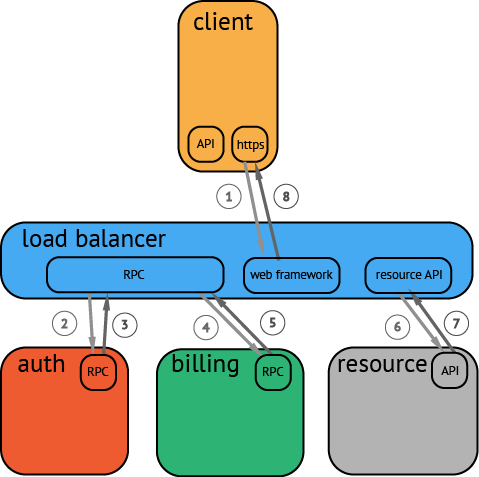
\includegraphics[width=\textwidth,height=6cm,keepaspectratio=true]{basic_trace}
\caption{A sample trace}
\label{basic_trace}
\end{figure}

\begin{figure}
\centering
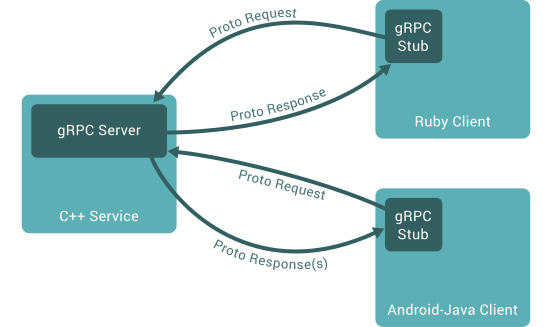
\includegraphics[width=8cm,height=6cm,keepaspectratio=true]{grpc_arch}
\caption{Architecture of gRPC}
\label{grpc_arch}
\end{figure}


\section{Background}
This section will provide an overview on Opentracing, the 
types of wire protocols that we explore for cross-process communication
and how annotations are propagated through them, and the reasoning behind 
integrating the fault injection mechanism into the tracing framework.


\subsection{OpenTracing}
Today's microservice architectures are large in scale and highly complex, often consisting 
of services written many languages; this makes distributed tracing over these services
extremely challenging. Opentracing\cite{opentracing:doc} provides a set of vendor-neutral
APIs for obtaining distributed traces through annotation propagation and allows for an easy
integration into existing microservice architectures. Previous solutions for tracing through
application level annotations such as Magpie\cite{magpie} and X-Trace\cite{xtrace} are unappealing
because of the per-application schema requirement and high overhead\cite{sigelman:dapper}. For these reasons,
we chose to use the Opentracing APIs to provide our architecture with fine-grained traces. 



\subsubsection{Trace Terminologies}
A \textbf{Span} is a basic, logical unit of work with a start time and duration, and exists within 
a single service; spans can be nested to show causal relation. A \textbf{Baggage} is a set of \textless K,V\textgreater pairs wrapped within a span's context, and allows for transparent propagation of arbitrary data. A \textbf{Tracer} consists of a set of Spans that belongs to a group of services; for example: a set of REST endpoints belonging to a group of services in a server. For cross-process tracing, a tracer will \textbf{inject} the span's context, and \textbf{extract} it on the other end.



\subsubsection{Trace flow}
Each service that a developer wishes to be traced will need to have a span constructed, after which it
will be added to a list of spans in the global tracer. Each span will automatically provide trace detail consisting of a timestamp and duration; the developer can decorate the span with more details, such as the status of a lock or value of a variable by adding to the span's baggage. When a service calls another service,
the tracer will have to be invoked to inject the local span's context into the wire, and extracted on the other side. During the extraction, a new(child) span is constructed from old(parent) span's context. Spans are recorded in the order that they are finished, meaning that whichever finishes first will be first to output trace information to the output stream. Figure \ref{basic_trace} shows a simple trace involving several microservices\cite{opentracing:doc}.


\subsection{Fault Handling}
There are three ways one could approach adding a fault injection component into a service consisting of
microservices, each of which have its own advantages and disadvantages over the other. The first way to approach this problem is to add the component in the services themselves, and each service will have its own chunk of code that will react accordingly as it receives information from upstream. The obvious advantage to this approach is that it is easy to implement and the developer has full control on how each service should react to a type of failure. However, this would mean that the code would have to be present in all the services, which could be a daunting task if there are tens if not hundreds of services written in a multitude of languages.

The second approach would be to have the wire protocol handle the fault itself. If all of the services are communicating through a single protocol, say HTTP, then this would greatly reduce the amount of coding that needs to be done in order to trigger faults. Even if the subsets of the services use different protocols, the amount implementation that needs to be done is proportional to the number of protocols used, which should be in the single digit. The downside to this approach would be the need to add an extension to the protocol, maybe even modifying core components in the protocol itself which could lead to bugs that might possibly violate the protocol's integrity.

The third approach would be to provide fault handling per programming language. This is the approach that we have chosen in our implementation, which will be provided in detail later on. This implementation is manageable in a sense that the number of languages in a service is bounded between ten and twenty, and we avoid the risk of polluting our code or the code of the wire protocol that we use. As an example, suppose we have a set of HTTP REST endpoints which are written in golang\cite{google:golang}, the only changes we need to make are to wrap our handler functions inside a decorator. Below is a code listing of how one would implement this:


\begin{lstlisting}[
    basicstyle=\tiny, %or \small or \footnotesize etc.
]

func homeHandler(w http.ResponseWriter, r *http.Request) {
    //stuff goes here
}

func decorate(f http.HandlerFunc) http.HandlerFunc {
    return func(w http.ResponseWriter, r *http.Request) {
        //do some preprocessing of the request
        f(w, r) //call the function
    }
}

func main() {
    http.HandleFunc("/home", decorate(homeHandler))

    http.ListenAndServe("localhost:8080", nil)
}
\end{lstlisting}

Notice that the changes to the application are minor, and that the decorator has full access to whatever was passed over the wire.



\subsection{Wire Protocols}
Wire protocols are used for writing application level code for cross-process communication. 
Protocols such as HTTP, gRPC\cite{google:grpc}, Thrift\cite{apache:thrift} provides a way for
services to receive data as they are called. Opentracing supports both HTTP and gRPC as wire protocols,
and uses them as a mean to propagate span context. In gRPC, clients specify methods that can be called 
remotely which the server will implement and handle client calls, and data is passed along gRPC wire in the 
form of Protocol Buffers\cite{google:protobuf}. The basic flow of the gRPC architecture\cite{google:grpc} can be seen in Figure \ref{grpc_arch}.



\subsection{Why integrate FI and tracing?}
We believe that fine-grained traces and request-level fault injection are complementary to one another.
One of the reasons we seek detailed traces in large scale, distributed services is to analyze a result
of a bad execution to find weak points that prevented a response to the client's request. It is on these
same weak points that we would like to inject faults to verify the failure in order for developers to fix.
Since Opentracing already provides a mean to easily pass arbitrary baggage between services, we would like
to take advantage of this and propagate request-level faults through baggage items. Of course, one could propagate such requests through the wire protocols themselves, bypassing the overhead of constructing spans and injecting them; however, the overhead of construction and injection are extremely small, and Opentracing's APIs allow for a clean way of handling the baggage data. 


%%%%%%%
%    EOF     %
%%%%%%%